%%%%%%%%%%%%%%%%%%%%%%%%%%%%%%%%%%%%%%%%%%%%%%%%%%%%%%%%%%%%%%%%%%%%%%%%%%%%%%%
%% 2020-06-20
%% Descr:       Hauptdatei für die Projektarbeit / Bachelorarbeit
%% Author:      Vorlage erstellt von Daniel Spitzer an der DHBW Lörrach 
%% Angepasst: Katja Wengler, ZWI, DHBW Karlsruhe
%%%%%%%%%%%%%%%%%%%%%%%%%%%%%%%%%%%%%%%%%%%%%%%%%%%%%%%%%%%%%%%%%%%%%%%%%%%%%%%

\newif\ifseminararbeit
\newif\ifblockingnotice
%%%%%%%%%%%%%%%%%%%%%%%%%%%%%%%%%%%%%%%%%%%%%%%%%%%%%%%%%%%%%%%%%%%%%%%%%%%%%%%
%% 2020-06-20
%% Descr:       Variablen für die Projektarbeit / Bachelorarbeit festlegen
%% Author:      Vorlage erstellt von Daniel Spitzer an der DHBW Lörrach 
%% Angepasst:   Katja Wengler, ZWI, DHBW Karlsruhe
%%%%%%%%%%%%%%%%%%%%%%%%%%%%%%%%%%%%%%%%%%%%%%%%%%%%%%%%%%%%%%%%%%%%%%%%%%%%%%%

% Hier müssen die Variablen zur eignenen Arbeit angepasst werden

% Der Titel der Arbeit, der auf dem Deckblatt angezeigt wird
\def \thesisTitle {Sentiment-Analyse der psychischen Gesundheit mit CRISP-DM}

% Der Titel der Arbeit, der in der Fußzeile angezeigt wird
\def \thesisFooterTitle {}

% Art der Arbeit
\def \thesisType {Projektarbeit DSKI}

% Bildungsabschluss
\def \degree {Bachelor of Science (B. Sc.)}

% Abgabedatum
\def \submissionDate {25. April 2025}

% Studiengang
\def \courseOfStudies {Data Science und Künstliche Intelligenz}

% Kurs
\def \course {WDS24B1}

% Name des Autors der Arbeit
\def \name {Björn Hilgers, Celine Lagler, Jihyun Yoo, Robbie Sumner}

% Name der Ausbildungsfirma
\def \company {}

% Ort, an dem Ausbildungsfirma ansässig ist
\def \companyLocation {}

% Betreuer der Ausbildungsfirma
\def \corporateAdvisor {Niklas Lederer, Stefan Eckerle}

% Wissenschaftlicher Betreuer
\def \universityAdvisor {}

% Ort und Datum für die Ehrenwörtliche Erklärung
\def \declarationHeading {Selbstständigkeitserklärung}
\def \declarationLocation {Karlsruhe}
\def \declarationDate {8. Dezember 2024}

% Ort und Datum für die Freigabe der Arbeit
\def \releaseLocation {Karlsruhe}
\def \releaseDate {8. Dezember 2024}

% Name der Bilddatei für das Firmenlogo. Die Datei muss im Ordner images sein.
% Erlaubt sind u.a. folgende Formate: PDF, PNG, JPEG
\def \fileNameLogo {company_logo.pdf}

% Je nach Länge des Titels kann die Schriftgröße angepasst werden
\def \titleFontSize {18}		% Schriftgröße des Titels auf dem Deckblatt
\def \footerFontSize {10}		% Schriftgröße in der Fußzeile

% Wenn es sich um eine Seminararbeit handelt,
% muss der folgende Befehl durch diesen ersetzt werden:
\seminararbeittrue
% \seminararbeitfalse

% Wenn die Arbeit keinen Sperrvermerk hat,
% muss der folgende Befehl durch diesen ersetzt werden:
\blockingnoticefalse
% \blockingnoticetrue

% Die Daten für den Sperrvermerk. Diese müssen natürlich nur geändert werden,
% wenn die Arbeit einen Sperrvermerk hat.
% Datum der Unterschrift des Autors auf dem Sperrvermerk
\def \blockingNoticeAuthorDate {31. August 2020}
% Datum der Unterschrift des Unternehmensvertreters auf dem Sperrvermerk
%\def \blockingNoticeCompanyDate {31. August 2020}

% Adresse und Land des Unternehmens auf dem Sperrvermerk. Die \\ sorgen für einen Zeilenumbruch
\def \companyAdress {Hauptstraße 1 \\ 76133 Karlsruhe \\ Deutschland}
% Telefonnummer des Unternehmens auf dem Sperrvermerk.
\def \companyPhone {0721 1234567}
% E-Mailadresse des Unternehmens auf dem Sperrvermerk.
\def \companyEmail {info@musterfrau-ag.de}
%%%%%%%%%%%%%%%%%%%%%%%%%%%%%%%%%%%%%%%%%%%%%%%%%%%%%%%%%%%%%%%%%%%%%%%%%%%%%%%
%% 2020-06-20
%% Descr:       Formale Einstellungen für die Praxisarbeit
%% Author:      Vorlage erstellt von Daniel Spitzer an der DHBW Lörrach 
%% Angepasst:   Katja Wengler, ZWI, DHBW Karlsruhe
%%%%%%%%%%%%%%%%%%%%%%%%%%%%%%%%%%%%%%%%%%%%%%%%%%%%%%%%%%%%%%%%%%%%%%%%%%%%%%%

\documentclass[a4paper,12pt]{article}
\usepackage{fontspec}
\usepackage{polyglossia}
\usepackage{csquotes}
\setdefaultlanguage[spelling=new, babelshorthands=true]{german}

% Seitenränder
\usepackage[left=3.5cm, right=2.5cm, head=1.25cm, bottom=2cm, foot=1.25cm, includefoot]{geometry}

% Abkürzungsverzeichnis
\usepackage[printonlyused]{acronym}

% Gut formatierte Tabellen
\usepackage{tabulary}
\usepackage{tabularx}  
\usepackage{array}

% Positioniert Tabellen und Abbildungen
\usepackage{float}

% Fügt Abschnitte wie den Anhang oder die Kurzfassung dem Inhaltsverzeichnis hinzu
\usepackage{tocbibind}

% Ermöglicht Abbildungen in LaTeX
\usepackage{graphicx}
\graphicspath{ {images/} }

% Definiert die Farben für Tabellen im DHBW-Style
\usepackage[table]{xcolor}
\definecolor{tableHeading}{gray}{0.672}
\definecolor{tableOdd}{gray}{0.945}
\definecolor{tableEven}{gray}{0.859}
\arrayrulecolor{white}

% Schriftart Carlito. Sie ist fast identisch mit Calibri.
% Calibri ist auf Linux und MacOS nicht verfügbar. 
\usepackage{carlito}
\setmainfont{carlito}

% Fußzeile und Kopfzeile
\usepackage{fancyhdr}
\renewcommand{\headrulewidth}{0pt}
\renewcommand{\footrulewidth}{0.5pt}
\def \footer{
{\centering
\fontsize{\footerFontSize}{\footerFontSize}\selectfont%\thesisFooterTitle
\thepage\par}
}



% Positioniert die Fußnoten fest am unteren Ende der Seite
\usepackage[bottom]{footmisc}

% Zeilenabstand: 1.5
\usepackage{setspace}
\setstretch{1.5}

% Literaturverzeichnis
\usepackage[natbib=true, backend=biber, style=authoryear, dashed=false]{biblatex}
\DeclareBibliographyAlias{interview}{misc}
\addbibresource{text/bibliography.bib}

% Das Paket hyperref muss als letztes Paket geladen werden. Das Paket setzt Links im PDF-Dokument.
\usepackage[hidelinks, unicode]{hyperref}
\hypersetup{pdftitle = {\thesisTitle}, pdfauthor = {\name}}

% Definiert die Farben für Code-Listings
\usepackage{xcolor}
\definecolor{RoyalBlue}{rgb}{0.25, 0.41, 0.88}
\definecolor{BrickRed}{rgb}{0.8, 0.25, 0.33}
\definecolor{OliveGreen}{rgb}{0.33, 0.42, 0.18}

% Code-Listings für Python
\setmonofont{sourcecodepro}
\usepackage{listings}
\lstset{
    basicstyle=\ttfamily\scriptsize, % Grundstil: Monospace, kleine Schrift
    frame=single, % Rahmen um den Code
    language=Python, % Programmiersprache: Python
    keywordstyle=\color{RoyalBlue}, % Schlüsselwörter: Weniger intensives Blau
    stringstyle=\color{BrickRed}, % Zeichenketten: Weniger intensives Rot
    commentstyle=\color{OliveGreen}, % Kommentare: Weniger intensives Grün
    showstringspaces=false, % Leerzeichen in Zeichenketten nicht anzeigen
    numbers=left, % Zeilennummern links
    numberstyle=\tiny\color{gray}, % Stil der Zeilennummern: Klein, grau
    breaklines=true, % Zeilenumbruch bei langen Zeilen
    captionpos=b, % Position der Beschriftung: Unten
}

% Normale Schriftart für URLs
\renewcommand{\UrlFont}{}

% Variable für das Speichern der Seitenzahl (römisch -> arabisch -> römisch)
\newcounter{pageNumber}

% Nummerierung: 2.1, 2.2 usw.
\renewcommand{\labelenumii}{\theenumii}
\renewcommand{\theenumii}{\theenumi.\arabic{enumii}.}

% Bei Bedarf können die Überschriften geändert werden
\def \declarationHeading{Selbstständigkeitserklärung}
%\def \thesisSizeHeading{Hinweis zum Umfang der Arbeit}
%\def \releaseHeading{Freigabe der Arbeit}
\def \blockingHeading{Sperrvermerk}
\def \abstractHeading{Kurzfassung}
\def \appendixHeading{Anhang}
\def \referenceHeading{Quellenverzeichnis}
\def \acronymHeading{Abkürzungsverzeichnis}

% Befehl für ein einleitendes Zitat
\newcommand{\epigraph}[2]{
    \begin{quote}\begin{quote}
        \begin{center}
            \textit{#1}
        \end{center}
        \hfill #2
    \end{quote}\end{quote}
}

\begin{document}
\thispagestyle{empty}
%%%%%%%%%%%%%%%%%%%%%%%%%%%%%%%%%%%%%%%%%%%%%%%%%%%%%%%%%%%%%%%%%%%%%%%%%%%%%%%
%% 2020-06-20
%% Descr:       Titelseite
%% Author:      Vorlage erstellt von Daniel Spitzer an der DHBW Lörrach 
%% Angepasst:   Katja Wengler, ZWI, DHBW Karlsruhe
%%%%%%%%%%%%%%%%%%%%%%%%%%%%%%%%%%%%%%%%%%%%%%%%%%%%%%%%%%%%%%%%%%%%%%%%%%%%%%%


\vspace*{-3cm}

\begin{center}


\includegraphics[width=6cm]{DHBW_logo.pdf}

\vspace{4cm}
\Large Fakultät Wirtschaft\\

\vspace{2cm}
\Large Studiengang \courseOfStudies \\

\fontsize{\titleFontSize}{\titleFontSize}\selectfont \thesisTitle \\

\vspace{1cm}
\thesisType \\

\normalsize Im Rahmen der Prüfung zum \degree \\

\ifblockingnotice
\vspace{0.5cm}
\Large \textcolor{red}{Sperrvermerk}\\
\vspace{0.5cm}
\else
\vspace{2cm}
\fi 

\submissionDate \\
\vfill
\end{center}

\begin{center}
    \begin{tabularx}{\textwidth}{|X|c|X|}
        Verfasser:innen: & \name \\
        Kurs: & \course \\
        % Dualer Partner: & \company, \companyLocation \\
        \ifseminararbeit
        \else 
        Betreuer: & \corporateAdvisor \\ 
        \fi
        Wissenschaftliche:r \\ Betreuer:in: & \universityAdvisor \\ 
        Abgabedatum: & \submissionDate \\
    \end{tabularx}
\end{center}
    
\pagenumbering{Roman}
\pagestyle{fancy}
\fancyhead{}
\fancyfoot{}
\fancyfoot[R]{\footer}
\newpage
%%%%%%%%%%%%%%%%%%%%%%%%%%%%%%%%%%%%%%%%%%%%%%%%%%%%%%%%%%%%%%%%%%%%%%%%%%%%%%%
%% 2020-06-20
%% Descr:       Eidensstattliche Erklärung
%% Author:      Vorlage erstellt von Daniel Spitzer an der DHBW Lörrach 
%% Angepasst:   Katja Wengler, ZWI, DHBW Karlsruhe
%%%%%%%%%%%%%%%%%%%%%%%%%%%%%%%%%%%%%%%%%%%%%%%%%%%%%%%%%%%%%%%%%%%%%%%%%%%%%%%

\section*{\declarationHeading}
\addcontentsline{toc}{section}{\declarationHeading}
\noindent Wir versichern hiermit, dass wir die vorliegende \thesisType mit dem Thema: 

%\begin{center}
\thesisTitle
%\end{center}

\noindent selbstständig verfasst und keine anderen als die angegebenen Quellen und Hilfsmittel benutzt habe. Wir versichern zudem, dass die eingereichte elektronische Fassung mit der gedruckten Fassung übereinstimmt.

\vspace*{1.8cm}

\begin{center}
    \begin{tabular}{@{}p{7cm}p{7cm}@{}}
        Karlsruhe, \declarationDate & \hrulefill \\
        & \name \\
    \end{tabular}
\end{center}
    
\newpage

\ifblockingnotice
%%%%%%%%%%%%%%%%%%%%%%%%%%%%%%%%%%%%%%%%%%%%%%%%%%%%%%%%%%%%%%%%%%%%%%%%%%%%%%%
%% 2020-06-20
%% Descr:       Sperrvermerk
%% Author:      Vorlage erstellt von Daniel Spitzer an der DHBW Lörrach 
%% Angepasst:   Katja Wengler, ZWI, DHBW Karlsruhe
%%%%%%%%%%%%%%%%%%%%%%%%%%%%%%%%%%%%%%%%%%%%%%%%%%%%%%%%%%%%%%%%%%%%%%%%%%%%%%%

\begin{center}
\section*{\textcolor{red}{\blockingHeading}}
\addcontentsline{toc}{section}{\blockingHeading}
\end{center}

\noindent Der Inhalt dieser Arbeit darf weder als Ganzes noch in Auszügen Personen außerhalb des Prüfungsprozesses und des Evaluationsverfahrens zugänglich gemacht werden, sofern keine anders lautende Genehmigung der Dualen Partners vorliegt.

\vspace*{2cm}


\newpage
\fi

% \section*{\abstractHeading}
\addcontentsline{toc}{section}{\abstractHeading}
Hier beginnt die Kurzfassung ihrer wissenschaftlichen Arbeit…
% \newpage

\tableofcontents
\newpage

\section*{\acronymHeading}
\newpage

\listoffigures
\newpage

\listoftables
\newpage

\clearpage
\setcounter{pageNumber}{\value{page}}
\pagenumbering{arabic}

\rowcolors{1}{tableOdd}{tableEven}

% -----------------------------------------------------
% Hier sind die Kapitel.
% Bei Bedarf kann man Kapitel entfernen oder hinzufügen
\section{Einleitung}

\subsection{Ausgangssituation und Motivation}
Die zunehmende Bedeutung sozialer Medien als Meinungsplattformen birgt Potenziale für datengetriebene Analysen öffentlicher Stimmungen. Unternehmen und Organisationen benötigen Werkzeuge, um relevante Diskussionen frühzeitig zu erkennen und einzuordnen. Technisch erfordert dies robuste Schnittstellen zu Plattformen wie Reddit sowie Methoden zur automatisierten Sprachverarbeitung (\emph{NLP} = Natural Language Processing).

\subsection{Projektidee und Anwendungsfall}
Ziel dieses Projekts ist die Entwicklung eines webbasierten Dashboards zur Analyse von Sentiment-Daten aus Reddit-Foren. Als Use Case dient die kontinuierliche Beobachtung gesellschaftlicher Diskurse, etwa in Bereichen wie Mental Health oder Produktfeedback. Die Anwendung richtet sich an Forschende, Journalist:innen oder Organisationen mit Interesse an digitalen Meinungsbildern.

\subsection{SMART-Ziele}
Das Projekt verfolgt klar definierte SMART-Ziele:
\begin{itemize}
    \item \textbf{Specific:} Entwicklung eines interaktiven Dashboards mit API-Anbindung und Sentimentanalyse.
    \item \textbf{Measurable:} Integration und Vergleich von Machine Learning-Modellen zur Sentimentanalyse; Visualisierung von (KPIs) Key Performance Indicators.
    \item \textbf{Achievable:} Bereitstellung einer benutzerfreundlichen Oberfläche.
    \item \textbf{Realistic:} Umsetzung im Rahmen eines studentischen Projekts.
    \item \textbf{Time-Bound:} Abgabe der lauffähigen Anwendung mit umfassender Dokumentation bis 2025.04.23.
\end{itemize}
\newpage
\section{Grundlagen}
%Dieses Kapitel könnte auch weg. Habe es vorsichtshalber drin gelassen.
\subsection{CRISP-DM und NLP–Pipeline}
Das Projekt folgt dem etablierten CRISP–DM–Modell, welches einen iterativen sechs­phasigen Prozess zur Lösung datengetriebener Aufgaben definiert:
\begin{enumerate}
    \item \textbf{Business Understanding}: Festlegung der Projektziele und Anforderungen.
    \item \textbf{Data Understanding}: Explorative Analyse der Rohdaten.
    \item \textbf{Data Preparation}: Aufbereitung und Transformation der Daten.
    \item \textbf{Modeling}: Anwendung verschiedener Machine–Learning–Algorithmen.
    \item \textbf{Evaluation}: Bewertung der Modellgüte anhand geeigneter Metriken.
    \item \textbf{Deployment}: Einsatz des finalen Modells zur produktiven Nutzung.
\end{enumerate}
Im Kontext der Sentiment–Analyse umfasst die NLP–Pipeline im Wesentlichen die Schritte:
\begin{itemize}
    \item Rohtextaufnahme und \emph{Cleaning} mittels regulärer Ausdrücke.
    \item Tokenisierung der Textdaten.
    \item Erzeugung numerischer Feature–Repräsentationen.
    \item Training und Test des Klassifikationsmodells.
    \item Bewertung und Interpretation der Vorhersagen.
\end{itemize}

\newpage

\subsection{Klassische Machine–Learning–Verfahren}
Für die Sentiment–Klassifikation wurden drei etablierte Algorithmen verglichen:
\begin{description}
    \item[K–Nearest Neighbors (KNN)]  
    Vergibt Labels basierend auf den $k$ nächsten Trainingsinstanzen. Wichtige Parameter: \texttt{n\_neighbors}, Distanzmetrik.
    \item[Decision Trees]  
    Hierarchische Partitionierung des Merkmalsraums. Splits erfolgen nach Gini–Impurity oder Entropie. Parameter: \texttt{max\_depth}, \texttt{min\_samples\_split}.
    \item[Random Forest]  
    Ensemble aus zufällig erzeugten Decision Trees, welches Overfitting reduziert und robustere Vorhersagen ermöglicht.
    
    Parameter: \texttt{n\_estimators}, \texttt{max\_depth}.
\end{description}
\newpage
\section{Data Understanding}

\subsection{Datenquelle und Struktur}
Die Datenbasis stammt aus einem öffentlich verfügbaren Datensatz auf Kaggle\footnote{\url{https://www.kaggle.com/datasets/suchintikasarkar/sentiment-analysis-for-mental-health}}. Die CSV-Dateien beinhalten mehrere zehntausend Social–Media–Posts, die jeweils einem der folgenden sieben mentalen Zustände zugeordnet sind:

\begin{itemize}
    \item \texttt{Normal}
    \item \texttt{Depression}
    \item \texttt{Suicidal}
    \item \texttt{Anxiety}
    \item \texttt{Stress}
    \item \texttt{Bipolar}
    \item \texttt{Personality Disorder}
\end{itemize}

Der Datensatz umfasst insgesamt 53.043 Einträge mit zwei Variablen: \texttt{statement} (ein Freitext) und \texttt{status} (eine kategoriale Zielvariable). Beide Variablen enthalten vereinzelt fehlende Werte. Zur Modellierung wurden die Daten in einen Trainingssatz (80\,\%) und einen Testsatz (20\,\%) unterteilt.
Die Daten wurden in einem \texttt{pandas} DataFrame geladen und die Spalten \texttt{statement} und \texttt{status} extrahiert. Die Spalte \texttt{statement} enthält den Freitext, während die Spalte \texttt{status} die zugehörige Klasse angibt.

\newpage

\subsection{Korpusbeschreibung}
Die Analyse des Korpus erfolgte hinsichtlich folgender Metriken:
\begin{itemize}
    \item \textbf{Word Instances}: Die Gesamtanzahl aller Token im gesamten Datensatz.
    \item \textbf{Word Types}: Die Anzahl einzigartiger Wörter nach Bereinigung.
    \item \textbf{Durchschnittliche Dokumentlänge}: Gemessen in Wörtern je Post.
\end{itemize}

Eine Initialanalyse zeigte eine hohe Varianz in der Textlänge (von <5 bis >100 Wörter) sowie eine ungleichmäßige Labelverteilung (Klassenungleichgewicht). 

\subsection{Visualisierung der Zielvariable}
Zur Untersuchung der Labelverteilung wurde ein Histogramm mit \texttt{Plotly Express} erstellt:

\begin{figure}[h]
    \centering
    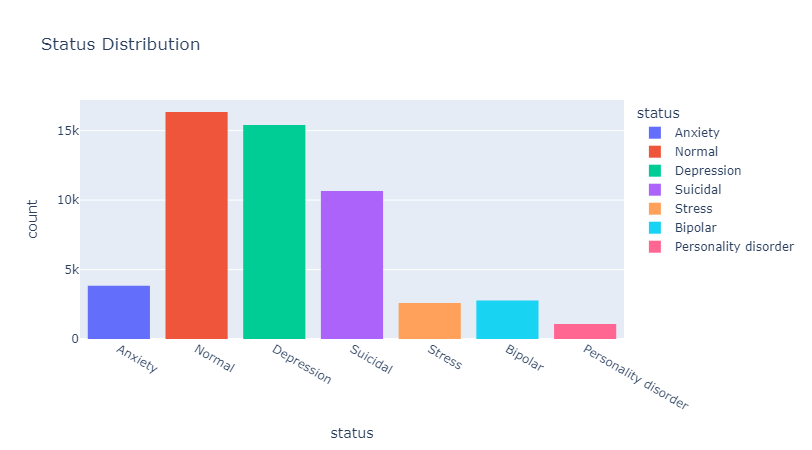
\includegraphics[width=0.75\textwidth]{images/class_distribution.png}
    \caption{Verteilung der mentalen Zustände im Datensatz}
    \label{fig:classdist}
\end{figure}

Die starke Dominanz der Kategorien \texttt{Normal}, \texttt{Depression} und \texttt{Suicidal} legt ein Klassenungleichgewicht nahe (z.\,B. Upsampling, Gewichtung bei Modellierung).


\subsection{Input– und Outputvariablen}
\begin{itemize}
    \item \textbf{Input}: Der bereinigte Fließtext aus der Spalte \texttt{statement}.
    \item \textbf{Output}: Die zugehörige Klassenvariable \texttt{label}, nominal skaliert.
\end{itemize}

\subsection{Prediction vs. Inference}
Die Zielsetzung dieses Projekts ist klar prognostischer Natur: Das Modell soll anhand unbekannter Social–Media–Texte automatisch den zugrundeliegenden mentalen Zustand erkennen. Dennoch sind auch inferenzielle Erkenntnisse möglich, z.\,B. welche Begriffe häufig in bestimmten Klassen auftreten oder welche Merkmale besonders trennscharf sind.

\subsection{Classification vs. Regression}
Die Klassifikation ist ein \textit{multinomiales Klassifikationsproblem}, da mehr als zwei Klassen vorhergesagt werden müssen.

\subsection{Korpusstruktur: N–Gramme}
Der aufbereitete Textkorpus umfasst insgesamt 5.961.315 Wortinstanzen (\textit{word tokens}) sowie 154.767 unterschiedliche Worttypen (\textit{word types}). Diese Kennzahlen geben Aufschluss über die Größe und Vielfalt des verwendeten Vokabulars.

\begin{figure}[h]
    \centering
    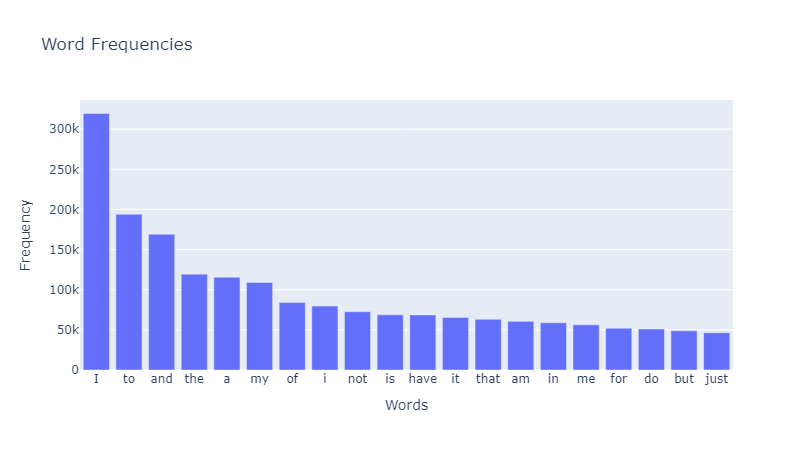
\includegraphics[width=0.75\textwidth]{images/word_frequencies.png}
    \caption{Häufigkeitsverteilung im Datensatz}
    \label{fig:wordfreq}
\end{figure}

Zur Beschreibung sprachlicher Muster wurden neben Unigrammen auch Bigramme betrachtet. Die häufigsten Bigramme (z.\,B. \textit{mental health}, \textit{feel like}) liefern semantische Hinweise auf häufig thematisierte Probleme.

\begin{figure}[h]
    \centering
    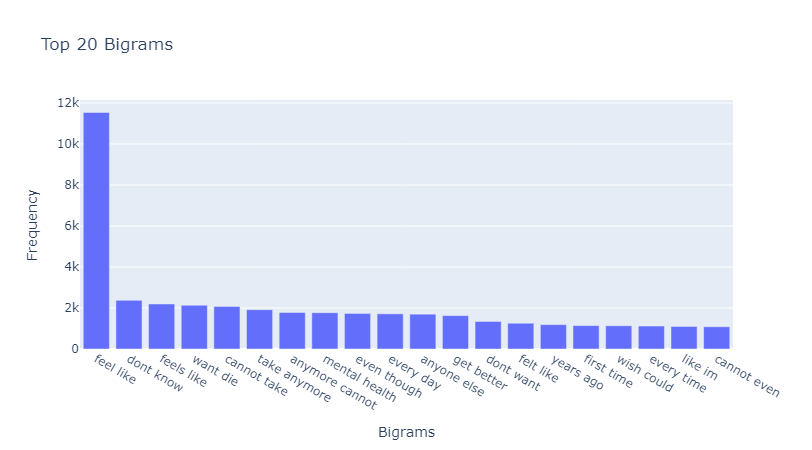
\includegraphics[width=0.75\textwidth]{images/bigrams.png}
    \caption{Verteilung der häufigsten Bigramme im Datensatz}
    \label{fig:bigrams}
\end{figure}

\subsection{Auffälligkeiten im Datensatz}

Bereits in der Phase des Data Understanding zeigten sich einige Auffälligkeiten:
\begin{itemize}
    \item Viele Texte enthalten HTML–
    
    Artefakte oder Sonderzeichen.
    \item Emojis, URLs und andere Rauschelemente stören die semantische Analyse.
    \item Die Labelverteilung ist stark unbalanciert,
    
    was die Modellgüte beeinträchtigen kann.
\end{itemize}
Diese Erkenntnisse flossen in die nachfolgende Vorverarbeitung ein.

\newpage

\subsection{Textvorverarbeitung}
Die manuelle Vorverarbeitung der Social-Media-Posts erfolgte in mehreren Stufen:

\begin{enumerate}
    \item \textbf{Kleinschreibung:}
    
    Im ersten Schritt der Textvorverarbeitung wurden alle Zeichen der Textvariable in Kleinbuchstaben umgewandelt, um die Konsistenz der Token zu gewährleisten und Redundanzen durch unterschiedliche Groß- und Kleinschreibung zu vermeiden:
        \begin{lstlisting}[language=Python, caption={Umwandlung in Kleinschreibung}]
        df["statement"] = df["statement"].str.lower()
        \end{lstlisting}

    \item \textbf{Regex-Cleaning:}
    
    Zur Bereinigung wurden reguläre Ausdrücke eingesetzt.
    
    Die folgenden Python-Befehle illustrieren den Ablauf und sind Beispiele aus dem Code. Für eine vollständige Liste der verwendeten Regex-Befehle siehe das Jupyter-Notebook im Anhang.

        \begin{lstlisting}[language=Python, caption={Regex-Cleaning der Social-Media-Texte}]
        
            # Entfernen von URLs
            df["statement"] = df["statement"].str.replace(r"https?://\S+|www\.\S+", "", regex=True)

            # Entfernen von mentions
            df["statement"] = df["statement"].str.replace(r"@\w+", "", regex=True)

            # Entfernen von HTML-Entities und Zero-Width Characters (z.B., "&#x27;", "\u200b")
            df["statement"] = df["statement"].str.replace(r'&#x[0-9a-fA-F]+;|\u200b', '', regex=True)
        \end{lstlisting}

    \item \textbf{Stopword-Entfernung:}

Zur Reduktion nicht-informativer Wörter wurden sogenannte \textit{Stopwords} entfernt. Hierzu wurde die englische Stopword-Liste aus der Bibliothek \texttt{nltk} verwendet. Jedes Token wurde überprüft und bei Übereinstimmung mit einem Eintrag der Stopword-Liste entfernt:

    \begin{lstlisting}[language=Python, caption={Entfernung englischer Stopwords mit nltk}]
        import nltk
        from nltk.corpus import stopwords

        nltk.download('stopwords')
        stop_words = set(stopwords.words('english'))

        def remove_stopwords(text):
            return ' '.join([word for word in text.split() if word.lower() not in stop_words])

        df["statement"] = df["statement"].apply(remove_stopwords)
    \end{lstlisting}

Nach Abschluss der Vorverarbeitung wurde der Korpus deutlich reduziert:

Er umfasst nun 2.717.728 Wortvorkommen (\textit{word instances}) und 76.395 unterschiedliche Wortarten (\textit{word types}).

Diese Reduktion verdeutlicht den Effekt der Reinigungs- und Filterprozesse auf die sprachliche Komplexität des Datensatzes. Obwohl der bereinigte Korpus nun ausschließlich relevante Terme enthält, bleibt die Anzahl der Worttypen hoch. Daher wird im nächsten Schritt eine weiterführende Tokenisierung eingesetzt, um die lexikalische Vielfalt weiter zu verringern.

    \begin{figure}[h]
        \centering
        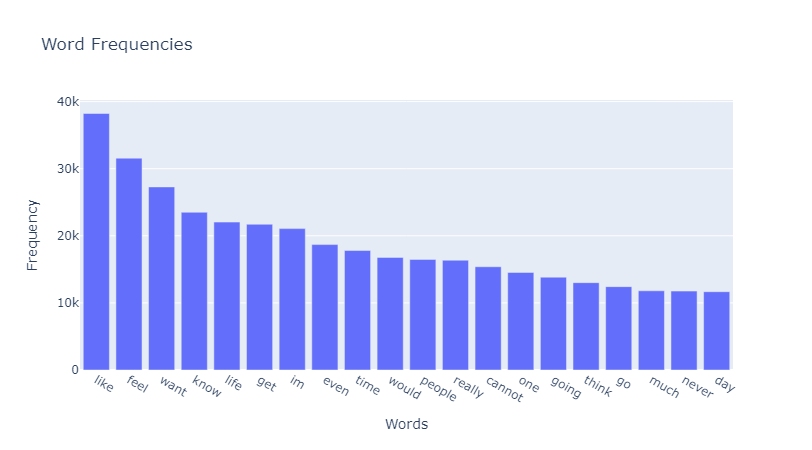
\includegraphics[width=0.75\textwidth]{images/new_word_frequencies.png}
        \caption{Verteilung der Wortinstanzen und -typen nach Bereinigung}
        \label{fig:newwordfreq}
    \end{figure}

    \item \textbf{Tokenisierung:}
    
Zerlegung der bereinigten Texte in einzelne Token durch Leerzeichentrennung 

mittels \verb|.split()| oder mit regulären Ausdrücken:

        \begin{lstlisting}[language=Python, caption={Tokenisierung mittels Regex}]
            tokens = re.findall(r"\w+", text)
        \end{lstlisting}

    \item \textbf{weitere Visualisierung:}
    
    Zur explorativen Analyse des Korpus wurde eine Wordcloud erstellt, welche die häufigsten Begriffe aus der \texttt{statement}-Spalte visuell hervorhebt. Dabei werden besonders häufig vorkommende Wörter größer dargestellt, während seltenere Begriffe kleiner erscheinen. Diese Form der Visualisierung erlaubt einen schnellen Überblick über zentrale Themen und sprachliche Muster im Datensatz. Zusätzlich wurden Wordclouds für verschiedene \texttt{status}-Kategorien generiert, um potenzielle Unterschiede in der Wortwahl zwischen den Klassen zu erkennen.

        \begin{figure}[h]
            \centering
            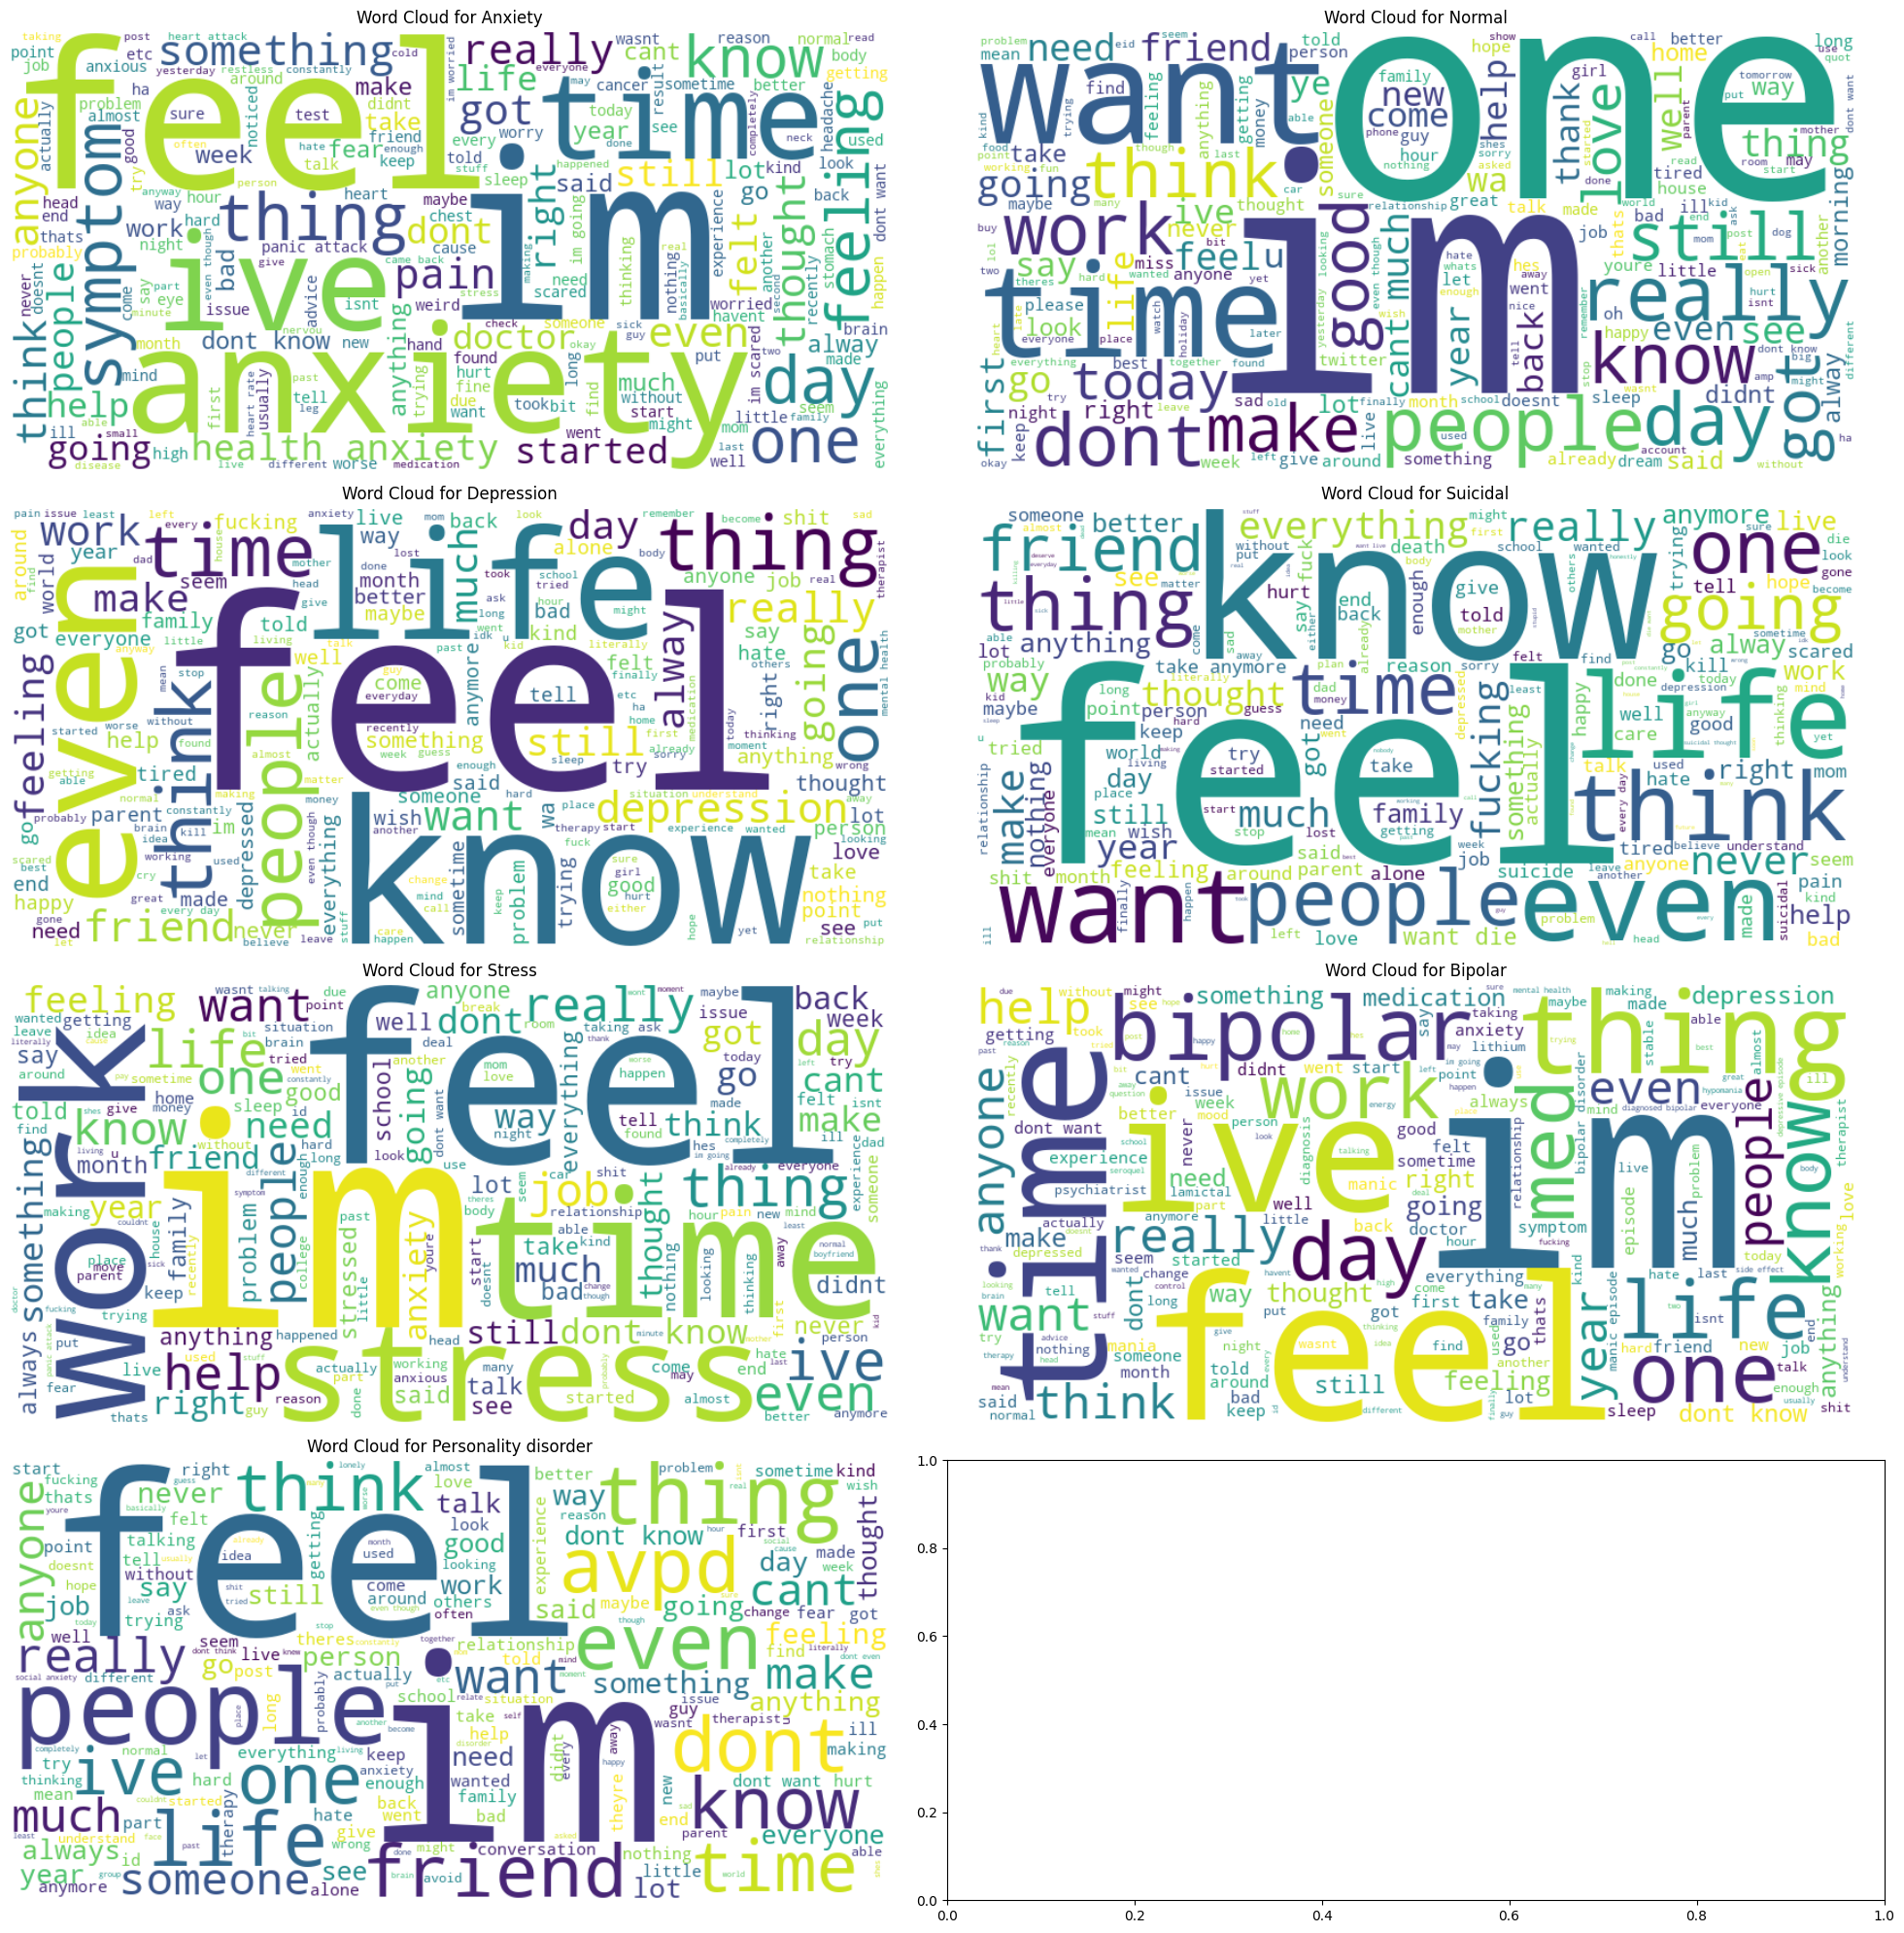
\includegraphics[width=0.75\textwidth]{images/wordcloud.png}
            \caption{Wordclouds für verschiedene \texttt{status}-Kategorien}
            \label{fig:wordcloud}
        \end{figure}

\end{enumerate}

\newpage

\subsection{Feature-Engineering: Bag-of-Words und N-Gramme}

Im Rahmen des Feature-Engineering-Prozesses haben wir das 

Bag-of-Words-Verfahren verwendet, um die Textdaten in numerische Repräsentationen umzuwandeln, die von Maschinenmodellen verarbeitet werden können. 

Das Verfahren basiert auf der Idee, dass Text als eine Sammlung von Wörtern betrachtet wird, ohne dabei auf die grammatikalische Struktur oder die Reihenfolge der Wörter Rücksicht zu nehmen. Dies ermöglicht es uns, die Häufigkeit von Wörtern in einem Text als Merkmale zu extrahieren, was für viele maschinelle Lernaufgaben nützlich ist.

Wir haben den \texttt{CountVectorizer} 

aus der \texttt{scikit-learn}-Bibliothek 

genutzt, um eine Merkmalsmatrix zu erstellen. 

Der \texttt{CountVectorizer} analysiert das Korpus und zählt, wie oft jedes Wort in den Dokumenten vorkommt. 

Durch die Auswahl von Monogrammen, also einzelne Wörter und Bigrammen, also Paare aufeinanderfolgender Wörter, wurde berücksichtigt, dass nicht nur einzelne Wörter, sondern auch Kombinationen von benachbarten Wörtern (wie z.\,B. mental health) wichtige Kontextinformationen für die Modellvorhersage liefern können.

Dies ermöglicht es, einfache semantische Beziehungen zwischen den Wörtern zu erfassen.

Um sicherzustellen, dass das Modell nicht nur auf den Trainingsdaten, 

sondern auch auf neuen, unsichtbaren Daten gut funktioniert, haben wir die Daten in

Trainings- und Testdatensätze aufgeteilt.

Dies geschah durch eine zweifache Anwendung von \verb|train_test_split|, um sowohl eine Modell als auch eine Validierungsaufteilung zu erzeugen. 

Der \verb|CountVectorizer| wurde dann auf den Trainingsdatensatz angewendet, um die Merkmale zu extrahieren und auf den Testdatensatz transformiert, um sicherzustellen, dass das Modell auf neuen Daten generalisieren kann.

Zusätzlich wurde die maximale Anzahl an Features auf 5000 begrenzt, um die Anzahl der Merkmale zu reduzieren und eine Überanpassung des Modells zu verhindern, was die Effizienz des Trainingsprozesses verbessert.
\newpage
\section{Modellierung}
\newpage
\section{Evaluation}

% -----------------------------------------------------

\label{pagesForDeclaration}

\clearpage
\pagenumbering{Roman}
\setcounter{page}{\value{pageNumber}}

\input{text/template/references}
\newpage

\section*{\appendixHeading}
\addcontentsline{toc}{section}{\appendixHeading}

\end{document}